%Short description of the posible actions in feedjam
FeedJam is a Twitter application that uses the Twitter REST API to retrieve data from Twitter. When entering the page the user can use the search field to search for their interests. The trending topics of the last 24 hours is also presented on the front page. Once the users has entered a search term the API's search method to retrieve tweets based on a query term. 
The system responds with relevant tweets from the last two weeks. It also retrieves information about the user that wrote the tweet. The application stores tweets, user information and trending topics in a database. 

Following we will give a more detailed desctiption of the appllication.

%Sections
\subsection{Structure}

\subsubsection{MVC} %torstein view delen, lisa model og contoller
The application is built on Spring's Web MVC framework. MVC separates the business logic from the user interface through the controller that handles the communication between the two. In Spring the dispatcherServlet...%blabla


\subsubsection{The Model} %what it does. what is contains 
The model is the part of the application that contains the domain objects or the core data structures \citep{}%find martin fowler
It 
Factory
We have data access objects (DAO) 
\subsubsection{The View}
The view is the component of MVC-applications which receives input from the user and displays output from the controllers and model. While the model and the controllers contain logic in order to do database interactions and data manipulation the view in general only contains logic in the form of simple if-statements and loops in order to display the content assigned by the controller. The view is also the component which, in web applications, contains the HTML markup, CSS-styling and javascript needed to provide users with the intentioned graphical design and user experience.

Within the context of Spring views are written in a language called JSP. JSP, Java Server Pages, is an alternative form of Java intended to be used within HTML and then compiled server side. While it is possible to write entire applications in JSP it is generally not considered good practice to do any logic outside logic specifically needed in order to display content from within the objects assigned to the view.

\subsubsection{The controller}
The controller takes the user input from the view and sends it to the business logic that handles it and sends response back to the controller.
In Spring the Controller prepares a Map which is sent to the 

%hva MVC er
%hvor ting er
\subsubsection{Interaction between view and controller} %snorre
\label{viewControllerInteraction}
When the user searches for a term on FeedJam a complex series of interactions happen between the view/the users browser and the FeedJam server. These interactions are illustrated in Figure~\ref{fig:AjaxInteractions}. When the user enters a search term into the FeedJam searchbox and clicks the search button the entered term is snapped up by Javascript. This search term is then along with some other variables formed into a GET request to the Twitter search API. The returned JSON is then sent to the AJAJ controller, which parses the JSON and generates a list of users whom are not in the database/or have not been updated for several weeks. This list of users is then returned to the client.

\begin{figure}[ht]
    \begin{minipage}[b]{1\linewidth}
        \centering
        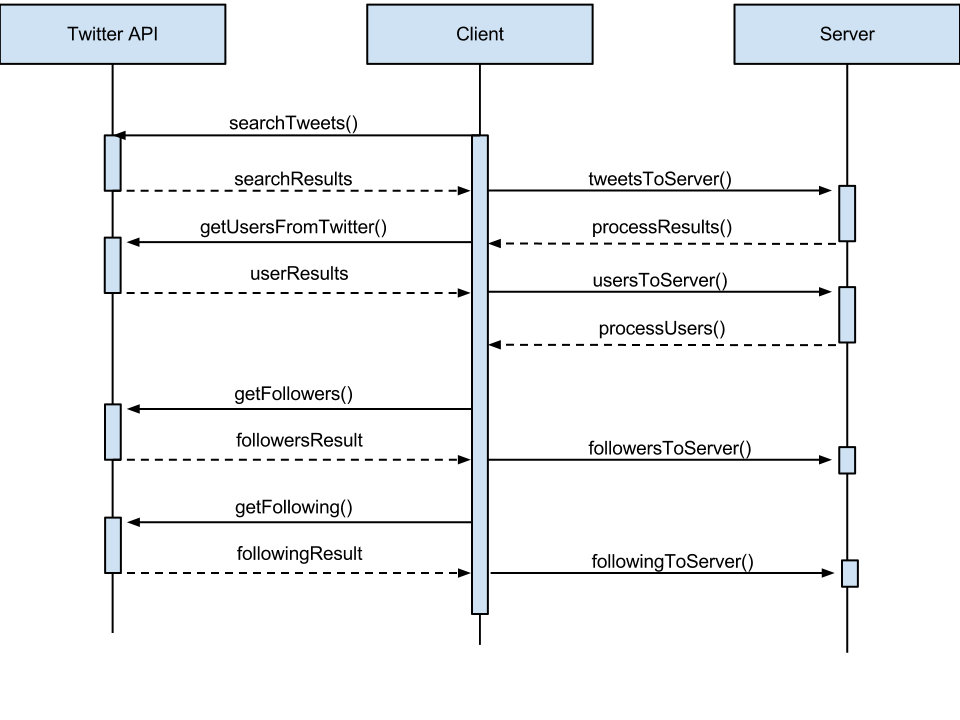
\includegraphics[width=1\textwidth]{figures/sequencediagram}
        \caption{Sequence diagram for ajax interactions between browser, server and Twitter.}
        \label{fig:AjaxInteractions}
    \end{minipage}
\end{figure}

\begin{figure}[h!]
\begin{lstlisting}[language=javascript]
// sends following to controller (ajaj/processFollowing)
function followingToServer(userId, followingData) {
  $.post("ajaj/processFollowing", 
  { 
    userId: userId.toString(), // server wants userId as a string
    following: JSON.stringify(followingData) // and JSON as a string
  },
  function(data) {
    console.log("SERVER RESPONSE: added following for " + userId);
  });
}
\end{lstlisting}
\caption{Example jQuery code for sending following for a user as JSON to the controller}
\label{ajaxRequest}
\end{figure}

The client then requests user information about all these users from Twitter. It then sends this back to the controller along with the returned tweets JSON from the previous request. The controller then processes all this and returns a finished view as HTML to the client. This finished HTML is then appended to the tweet grid.

After the generated view has been inserted the client starts requesting followers and following for each of the users who were looked up. This is done this lately in the process in order to ensure that the view is returned and displayed to the FeedJam user as soon as possible in order to make the system appear faster, through using AJAX this can also be done without the user noticing. Each response from the Twitter API is then asynchronously send to the controller which in turn processes the JSON and inserts the values into our database.

\subsubsection{Interaction between controller and model} %lisa
%information flow, hvordan ting skjer
FeedJam has tree controllers. The HomeController handles the trend requests for from the front page. It finds the time of the request and uses the MySQLTrendingFactory class to search the database for trends. If the trend exist in the database they are returned to the view. If trends for the current hour don't exist in the DB, a request is sent to Twitter. The response is cached and sent to the view. More on the database structure in section \ref{feedJamDatabase} \nameref{feedJamDatabase}.

AjajController handles all search requests. When the client has retrieved search results from Twitter, the Json response is posted to AjajController. Using the MySQLUserFactory, it queries the database to check if user information of the tweet owners is cached. If some users don't exist in the database, a response is sent to the view. It contains a Json array of users the client needs to retrieve information about. 

The AjajConntroller then receives a POST containing the the information on the remaining users information. New users and the Tweets are inserted to the database and a TweetSearchResult object is created. The result contains the requested Tweets with associated user information. The result is then sent as a response to the view. When the client has received the response from the server it requests the users followers and following. The list containing these users is sent to AjajController which uses MySQLUserFactory to inserts them to the database. The application logic for this operation is listed in Figure \ref{javaProcessFollowing}

\begin{figure}[h!]
\begin{lstlisting}[language=java]
@RequestMapping(value = "/processFollowing", method = RequestMethod.POST)
public ResponseEntity<String> processFollowing(
  @RequestParam String userId,
  String following) 
  {
    long userIdLong = Long.parseLong(userId);
    
    // Parse the json string and store following in result page object
    FollowersFollowingResultPage followingResultPage = 
      JsonUserParser.jsonToFollowersFollowing(userIdLong, following);
    
    // Insert following objects into database
    int updated = 
    mySqlUserFactory.insertBatchFollowing(followingResultPage);

    // Return a HTTP OK status to the client				
    return new ResponseEntity<String>(HttpStatus.OK);
}
\end{lstlisting}
\caption{Example Java code for receiving and inserting following into the database.}
\label{javaProcessFollowing}
\end{figure}

The SearchController is now used as a back up. It originally handled server side requests to Twitter. As explained in section \label{twitterProblem} we had a large amount of problems connected with the limited amount of requests per ip-adress per hour. Since the SearchController performed API requests server-side this meant that FeedJam could serve a maximum of 150 searches per hour in total. While all API requests are handled client-side in the final FeedJam version we keep the SearchController as a backup in the cases where the users have disabled Javascript in their browser in order to provide a similar, though limited, experience for those users.

%brukt desingn patterns 

{\bf packages}
\begin{itemize}
  \item uib.info323.twitterAWSM contains the controllers
  \item uib.info323.twitterAWSM.exceptions contains exceptions
  \item uib.info323.twitterAWSM.io contains interfaces for interacting with persistence layer (postfixed -DAO), interfaces for searching the Twitter API (postfixed -SearchFactory) and interfaces for crating model object (postfixed -Factory).
  \item uib.info323.twitterAWSM.io.impl contains MySql implementations, Json implementations and model implementations. 
  \item uib.info323.twitterAWSM.io.rowmapper contains rowmappers used in accessing persistence layer
  \item uib.info323.twitterAWSM.model.impl contains model implementations
  \item uib.info323.twitterAWSM.model.interfaces contains model interfaces
  \item uib.info323.twitterAWSM.model.impl contains model implementations
  \item uib.info323.twitterAWSM.pagerank contains PageRank/UserRank implementation
  \item uib.info323.twitterAWSM.model.utils contains parsers etc.
\end{itemize}


\subsection{Layout} %torstein
A large part of our project was to develop a novel way of displaying tweets. This section will explain how we developed the layout concept in addition to explaining how we implemented it using modern standards and techniques.

\subsubsection{Defining the concept}
Since FeedJam is an effort to ease the consumption of tweets and Twitter conversations through the use of the Page Rank algorithm to rank users and a simple tweet ranking we needed a good way of displaying the results of said rankings graphically. Normally search engines are able to sort the output of searches after relevance due to their non-restricted access to their own database. However, in the case of Twitter we only have access to a severely limited number of tweets through their public API. In addition to this we believe that the shere amount of new tweets every minute would be a too large amount to effectively process for our computers and server even if we were able to fully access the Twitter database. Therefore a normal sorted listing of search results were rendered effectively impossible. Another aspect to take into consideration is the conversational nature of many tweets. It was decided that the FeedJam layout would somehow follow the conversation without sorting tweets but simultaniously helping users skim through large conversations quickly and help users see important tweets.

Normally when browsing through lists of unsorted rated content we are explicitly shown the content's rating. This is true for instance in the case of movie or music listings where a grade is displayed, often in the form of a dice or a number. While we did want to display our rating we also wanted to provide the user with more powerfull visual cues to the generated importance measure of tweets in order to follow our layout goal of easing skimming of large conversations. Hence we decided on the use of purely visual cues in the form of colours or transparency in order to differentiate between rankings.

\subsubsection{Early efforts}
Early concepts placed tweets in a list format. The thinking behind using a simple list format is that Twitter in its current iteration use a similar design to display tweets. This did however prove to be an inefficient use of the available space in the browser, and was quickly scrapped in favour of a grid-based layout.

\begin{figure}[ht]
    \begin{minipage}[b]{0.5\linewidth}
        \centering
        
\includegraphics[width=\textwidth]{figures/twitter_list}
        \caption{Twitter in its current iteration.}
        \label{fig:Twitter}
    \end{minipage}
    \hspace{0.5cm}
    \begin{minipage}[b]{0.5\linewidth}
        \centering
        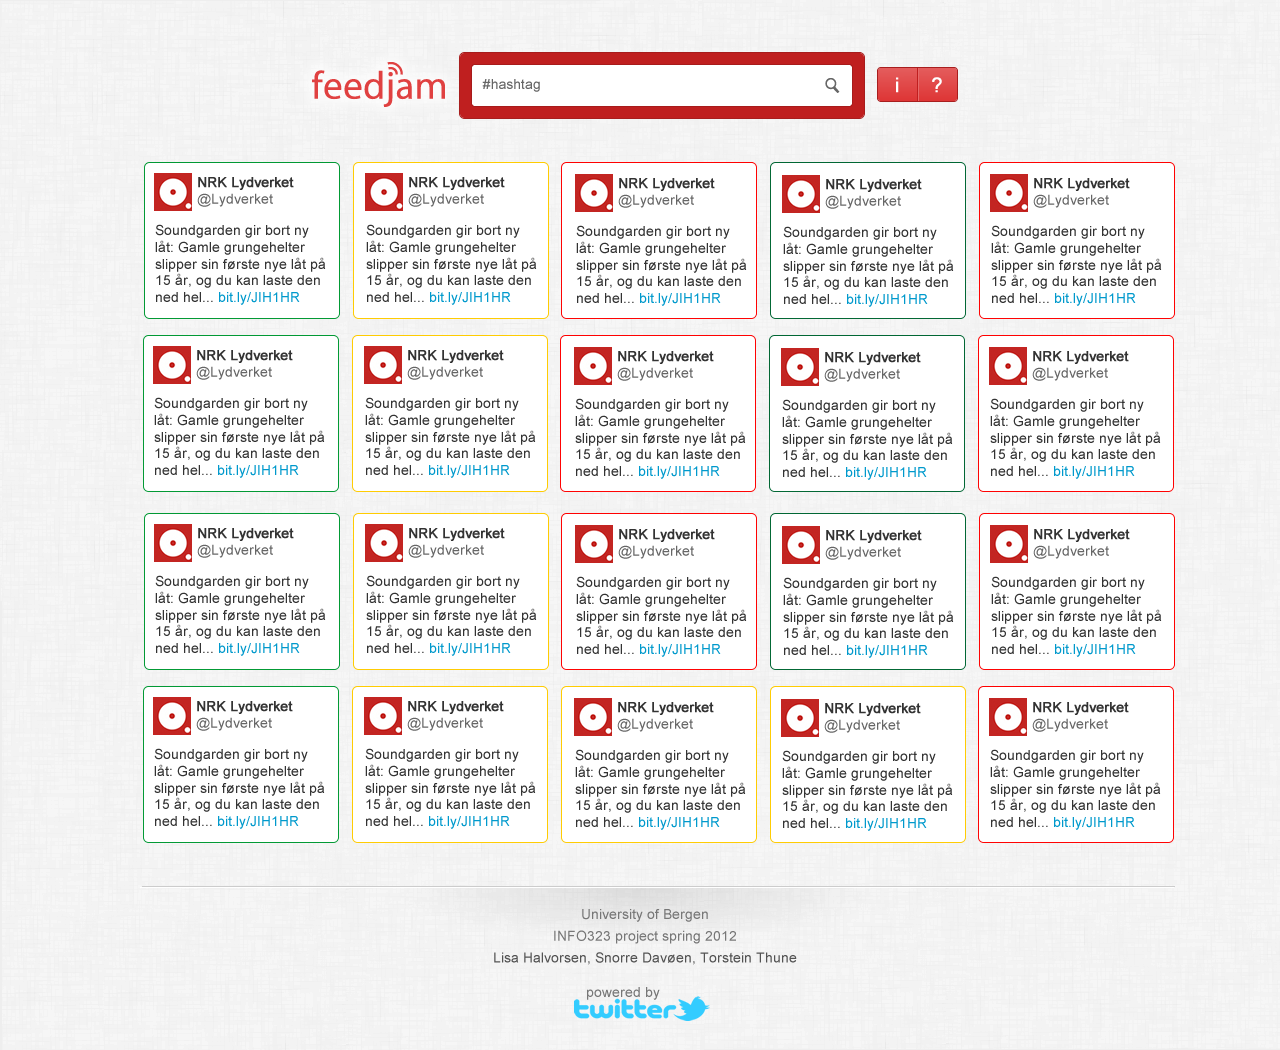
\includegraphics[width=\textwidth]{figures/layout_colour_borders}
        \caption{Early FeedJam concept}
        \label{fig:FeedJamColours}
    \end{minipage}
\end{figure}

We did also experiment with using colours to display the importance of tweets. Early thoughts used a traffic light metaphor where green signalised a good ranking, yellow a neutral ranking and red a bad ranking. The colours were used as border colours, as seen in figure  \ref{fig:FeedJamColours}. This did however prove to be a too insignificant visual cue, as in it took too long time for us to actually determine the rating of tweets through tis colour use, we also decided that the colours cluttered the design, making it less aestethical. Another problem was that we were only able to create three ranking brackets using our traffic light metaphor, which took away from the nuances of our ranking algorithm.

\begin{figure}[ht]
    \begin{minipage}[b]{1\linewidth}
        \centering
        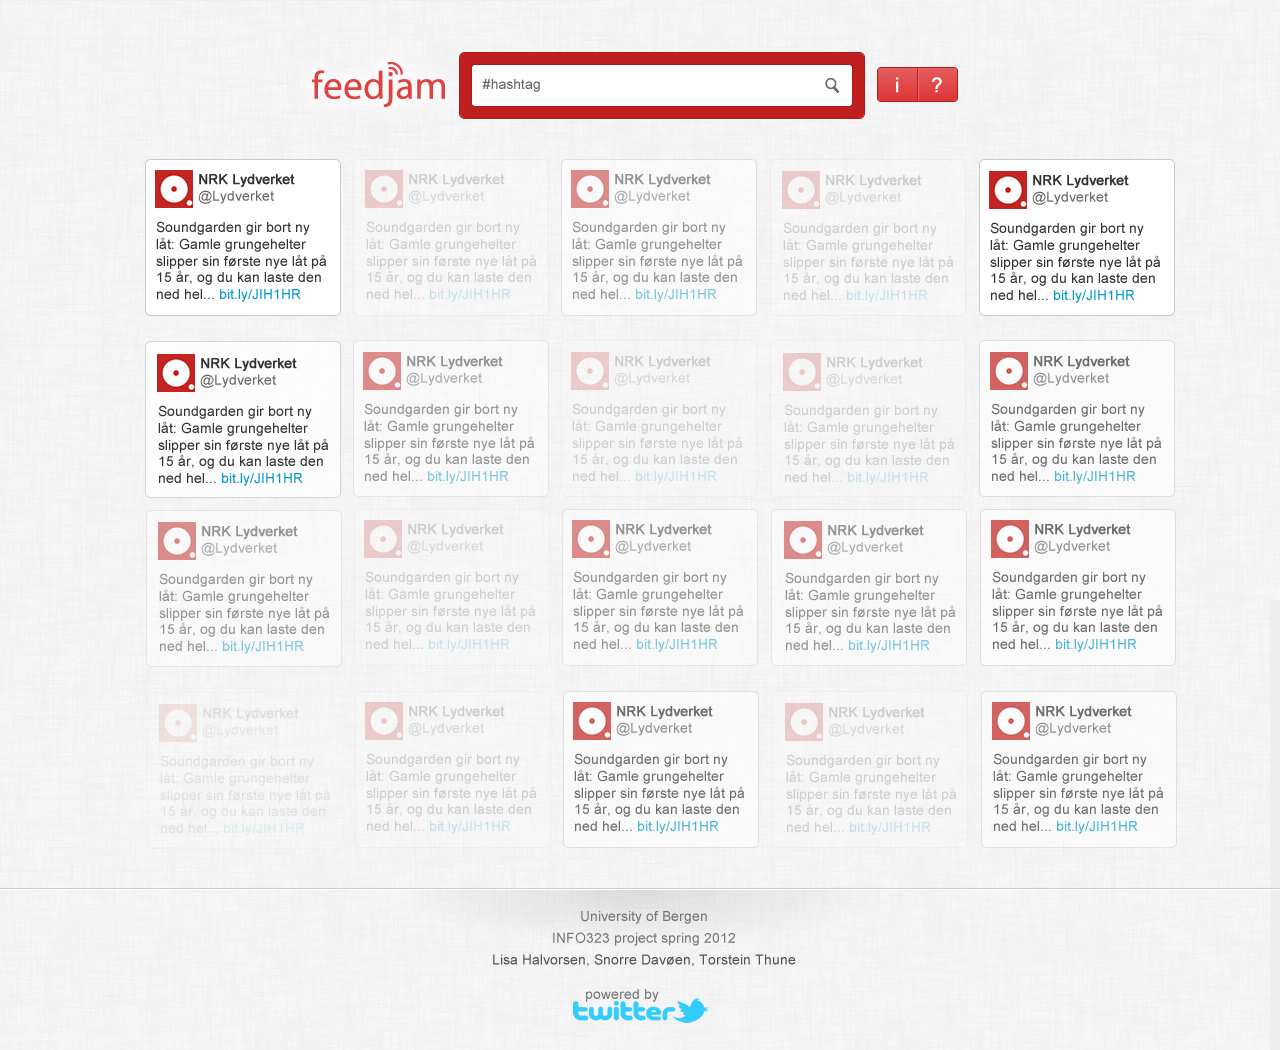
\includegraphics[width=0.5\textwidth]{figures/layout_transparency}
        \caption{FeedJam concept using transparency}
        \label{fig:FeedJamTransparency}
    \end{minipage}
\end{figure}


Since our ranking algorithms has an output in the form of a float number (a number betweet 0.0 and 1.0) we decided that opacity, whose CSS operator can take in values in a float format, would be better since we would be able to display the nuances of our ranking algorithm to within two decimals.


\subsubsection{The final layout}
When visiting the FeedJam web application the users are presented with a clean layout consisting of a logo, a search box, a list of trending tweets and a footer containing some information about the project and its creators. The colour scheme is very simplistic, relying on red and different shades of gray, resulting in a minimalistic design.

\begin{figure}[ht]
    \begin{minipage}[b]{0.5\linewidth}
        \centering
        
\includegraphics[width=\textwidth]{figures/feedjam_final_frontpage}
        \caption{FeedJam frontpage on laptop/desktop computers}
        \label{fig:FeedJamFrontpage}
    \end{minipage}
    \hspace{0.5cm}
    \begin{minipage}[b]{0.5\linewidth}
        \centering
        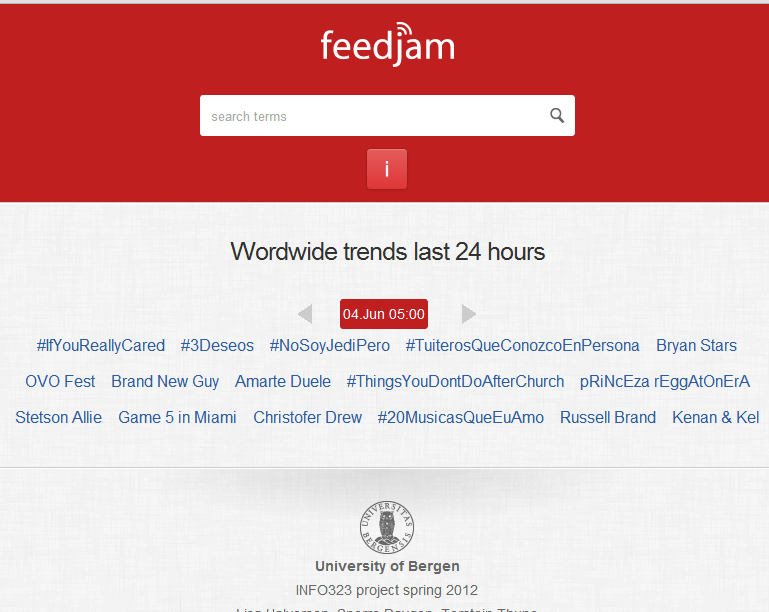
\includegraphics[width=\textwidth]{figures/feedjam_responsive_frontpage}
        \caption{FeedJam frontpage on tablets}
        \label{fig:FeedJamFrontpageTablet}
    \end{minipage}
\end{figure}

The search form consists of a standard, though large, search input field and a search button, thus providing both good visibility, since the form is very prominent, and affordance, since users are used to the concept of a search box and thus knows how to use it.

When entering a search term and clicking the search button (or when clicking a trending topic) the front page fades out, and a loading bar appears displaying information about what is being done, which is further explained in section \ref{viewControllerInteraction}. While the site exhibits unusual form behaviour, e.g not causing a page reload when clicking submit, this loading bar, with its connected loading messages, shows the user that something has happened and that something is still happening, thus fulfilling the feedback design principle.

\begin{figure}[ht]
    \begin{minipage}[b]{1\linewidth}
        \centering
        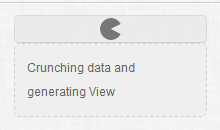
\includegraphics[width=0.5\textwidth]{figures/feedjam_loading}
        \caption{The loading bar}
        \label{fig:FeedJamLoading}
    \end{minipage}
\end{figure}


The search result page consists of a strict grid with 4 columns (or less depending on screen resolution) where each tweet is set at a specific width. Each tweet is in its own box with varying opacity depending on the relevant rankings. In order to more clearly show where tweets are in the grid even on lower opacities the border is always at 100\% opacity. While some tweets are almost transparent they will become fully visible when pointed at by the mouse pointer or clicked on tablets and smart phones in order to make them readable.

When clicking a username a small modal window appears displaying information about the user, including our user rank, the number of people following the user and the number of people followed by the user, the user's description from Twitter and links to his/her web page and profile. This window can be closed either by clicking the user name itself or by clicking outside the modal window.

Beneath the grid of tweets there is a "load more" button. By clicking this button the user sends an AJAX request both to twitter to get the next 20 tweets which is then sent to the server. The server in turn goes through the same steps as when using the search box, finally resulting in a generated view (a tweets grid) which is dynamically appended to the existing grid using jQuery.


\subsubsection{Coding of the layout}
The frontend is coded using standard HTML5 for markup/structure, CSS3 for styling and Javascript coupled with jQuery for front-end scripting. In addition we use JSPs, which are in essence compiled template files, to generate the HTML displayed to the user.

The frontend is organised in several views. Roughly we can divide these views into two categories: main views and views which are included into other views. FeedJam has one main view called home.jsp. This view is generates the markup which the user is presented with when he/she first visits the feedjam website. The home view also uses the views footer.jsp which contains the markup for the footer (bottom of page), htmlheader.jsp which contains javascript declarations and jQuery initialisation and header.jsp which contains the search form. Other views is the tweetList.jsp view and the trendingList.jsp view which are used to generate grids of tweets and a slider of trending topics. These are placed dynamically within the home.jsp view through the use of jQuery.

%Backend: Spring, Spring mvc, maven,  DAO, factorys, running on java servers, db more in db section,  developement
%\subsection{Backend} %Serverside?
%The application is developed in Spring MVC framework. 

%Ranking: implementation, reference
\subsection{Ranking} %lisa
\label{ranking}
The FeedJam ranking consist of two parts, the TweetRank and the UserRank. It's displayed through the opacity of each tweet. The idea is that tweets tweeted by a user with high UserRank gets a good score. The tweet will have close to 100\% opacity (no transparency) unless the tweet itself does not contain spam signals (see more below). The FeedJam ranking will also allow for normal users who follow good tweeting practice to get a good score.

\subsubsection{TweetRank}
The TweetRank is based on the idea of using ranking signals in search engines. Even though there isn't as many content signals in a tweet as in a normal web pages we use them to make the TweetRank. "\#" symbol is used in Twitter to mark keywords or topics in a tweet \citep{Twitter}. Twitter recommends using no more than 2 hash tags in a tweet. 
Mentions are another mark-up that's used in tweets. It indicates either that a tweet is a reply to another tweet or that a tweet concerns a user \citep{Twitterb}. If a Tweet is read by many, it is considered important. The Twitter API does not provide this statistic. We have decided to use the retweet count of tweets as a heuristic to get an idea of how many times a tweet might have been read.

\subsubsection{UserRank}
The UserRank use information about a user's followers and who a user follows to rank the user. The follower relation between to users represent the back-link (or inbound link) relationship in a page rank algorithm. The following relationship between two users represent the forward link (or outbound link) relationship. If the reader recalls the three user categories described in section~\ref{Twitter}, it is clear that a user with a high user rank (i.e. high page rank) falls under the category Information source, and should therefore be regarded as an interesting user. It is probable that a highly ranked user have many followers, the followers themselves having a high user rank, because she makes interesting tweets.

{\bf UserRank implementation}\newline
The UserRank implementation used in FeedJam is based on \citet{Goodrarzi2009}'s implementation of page ranking in Java. The first step when finding a user \emph{a}'s UserRank is to find all the followers of the user, then find their followers. This is repeated to all related users is found and stored in a list (params). A matrix is then generated from the users in the params-list. Then a matrix containing a multifactor-constant is created. The multifactor is calculated based on the relations between the users, how many are following them and the damping factor (see source code UserRank.getMultiFactor). After this a matrix of 1- DAMPING\_FACTOR is made. These two matrixes makes out the linear equation that is the user's UserRank. The solving of the equation is left to a third party API \citep{Jama}. Lastly the rank of the user is picked out of the matrix.

%Litt mer om hvordan pagerank kan brukes på Twitterusers. Lage en graph/tegning. Vise at det i teorien skal oversettes - argumentere. Sosiale nettver er ganske like weben. 
%Optimalisation 
Our initial implementation of the ranking algorithm was extremely slow and ranking every user was simply  not feasible with the time requirement of the algorithm. To optimize the algorithm we performed some simple time complexity analysis to identify critical operations in the ranking algorithm which could be optimized. To explain how we optimized the algorithm it is necessary to show some of the source code used in the ranking algorithm. Figure~\ref{fig:generateMatrix} shows the code that generates the matrix used in the algorithm. The generateMatrix method gets the multi factor for each cell in the matrix. The getMultiFactor method is run \(n^2\) times where n is the number of users in the parameter list.

\begin{figure}[h!]
\begin{lstlisting}[language=java]
private double[][] generateMatrix(){ 
  double[][] arr = new double[params.size()][params.size()]; 
    for(int i = 0; i < params.size(); i++){ 
      for(int j = 0; j < params.size(); j++){ 
        arr[i][j] = getMultFactor((String) params.get(i), (String) params.get(j));
      }
    } 
  return arr;
}
\end{lstlisting}
\caption{Java code for generating the linear equation parameter matrix \protect \cite{Goodrarzi2009}.}
\label{fig:generateMatrix}
\end{figure}

If one takes a close look at the original getMultiFactor method (Figure~\ref{fig:getmultifactor}) one can see that two database operations, getInbound and getOutBound, are performed for each matrix cell. This amounts to a time complexity of O(\( n^2\)) for these two database operations. If one presupposes that each database operation takes about 50 milliseconds to complete, then the time requirement of a user with a param list of 1000 users would be  \((1000^2 \cdot 50) \cdot 2\) milliseconds, which is about 1666 minutes. To optimize the algorithm we moved both database operations outside the double for-loop, thereby reducing the time-complexity of these operations to O(n) which is an significant improvement (Figure~\ref{fig:getmultifactorimproved}). Using the example above the time requirement would now be \(1000 \cdot 100\) which is 100 seconds. Calculating the multi factors is still a \(n^2\) problem, but every value is now in memory which should reduce the time used by the function. While this optimization does consume more memory, the additional memory consumption is negligible compared to the vast reduction in computing time.

\begin{figure}[h!]
\begin{lstlisting}[language=java]
private double getMultFactor(String sourceId, String linkId){ 
  if(sourceId.equals(linkId)) 
    return 1;
  else{
    String[] inc = getInboundLinks(sourceId); 
    for(int i = 0; i < inc.length; i++){ 
      if(inc[i].equals(linkId)){ 
        return -1 *(DAMPING_FACTOR / getOutboundLinks(linkId).length);
      } 
    }
  } 
  return 0;
}
\end{lstlisting}
\caption{Java code for calculating the multi factors used in the linear equation parameter matrix \protect \cite{Goodrarzi2009}.}
\label{fig:getmultifactor}
\end{figure}

\begin{figure}[h!]
\begin{lstlisting}[language=java]
private double getMultiFactor(
  long sourceId, 
  long linkId, 
  Map<Long, Long[]> followers, 
  Map<Long, Integer> allNumberOfFollowing) 
  {
  if (sourceId == linkId) {
    return 1;
  } else {
    for (long follower : followers.get(sourceId)) {
      if (follower == linkId) {
        double factor = 0;
        try {
          long start = System.currentTimeMillis();
          factor = -1 * (DAMPING_FACTOR / allNumberOfFollowing.get(linkId));
        } catch (ArithmeticException ae) {
          return DEVIDED_BY_ZERO;
        }
        return factor;
      }
    }
  }
  return 0;
}
\end{lstlisting}
\caption{Improved getMultiFactor-method with reduced time-complexity for the database-operations.}
\label{fig:getmultifactorimproved}
\end{figure}

%caching DB 
\subsection{Database} %lisa
\label{feedJamDatabase}
The application uses a MySQL database to store information from Twitter. This was necessary because the Twitter API has restrictions on number of request one can make to it.
We user the DAO pattern to create an abstraction between the domain objects and the datasource.  The DAO interfaces TrendDAO, TweetDAO and UserDAO defines the operations that are alowed to do.  


\citep{boka kap11} caching is used in search engines a a means for making the search engine be or seem faster. we do caching of Twitter information. We desided to implement chariang of information from twitter because of the restriction on requests problem (see section \ref{} \nameref{}) 

We could also have used caching of query results. store the result of one query, but wouldnt have the oppdaterthet %
one of the features of Twitter search. could have beenn used in some other function in the application like looking at the history of tweets. \citet{boka kap 11, under caching} sais that 50\% is cached

%Litt mer om hvordan pagerank kan brukes på Twitterusers. Lage en graph/tegning. Vise at det i teorien skal oversettes - argumentere. Sosiale nettver er ganske like weben. 

%Optimalisation 
cs430 users 
before optimalization
1650 sek
after first optimalization
8 sek

%caching DB 
\subsection{Database} %lisa
\label{feedJamDatabase}
The application uses a MySQL database to store information from Twitter. This was nececary because the Twitter API has restrictions on number of request one can make to it.
We user the DAO pattern. The DAO pattern is used as an abstraction of the connection between the domain objects and datasource. The DAO interfaces TrendDAO, TweetDAO and UserDAO defines the operations that are alowed to do.  


\citep{boka kap11} caching is used in search engines a a means for making the search engine be or seem faster. we do caching of Twitter information. We desided to implement chariang of information from twitter because of the restriction on requests problem (see section \ref{} \nameref{}) 

We could also have used caching of query results. store the result of one query, but wouldnt have the oppdaterthet %
one of the features of Twitter search. could have beenn used in some other function in the application like looking at the history of tweets. \citet{boka kap 11, under caching} sais that 50\% is cached




